\documentclass[11pt,a4paper]{ctexart}
\usepackage[top=1in,bottom=1in,left=1.25in,right=1.25in]{geometry}
\usepackage{graphicx}
\usepackage{tikz}
\usepackage{times,bitmetr}
\usepackage{algorithmic}
\usepackage{algorithm}
\usepackage{array}
\usepackage{mdwmath}
\usepackage{mdwtab}
\usepackage{amsmath}
\usepackage{amsfonts}
\usepackage{amssymb}
%\usepackage{anysize}
\usepackage{subfigure}
\usepackage{pifont}
\usepackage{color}
\usepackage{float}
\usepackage{soul}
\usepackage{tabu}
\bibliographystyle{IEEEtran}



\title{Research Report Two}
\author{Xinpeng Hong
	\thanks{The author acknowledges the support of wavelab in
		making this project a reality}\\
	\\\\
}



% Change to the current month of the series
\reportmonth{October 1}
% Change to the current year of the series
\reportyear{2019}
% Change to the TR number that you obtained from the
% UWEETR web pages when you initially created a new
% TR number. Only provide the last 4 digits here, the year
% goes in the \reportyear{} field above.
\reportnumber{0002}



\begin{document}
\makecover
\maketitle
	

\section{SeqGAN论文阅读与理解}
\subsection{标题}
\noindent SeqGAN: Sequence Generative Adversarial Nets with Policy Gradient
\subsection{动机}
\noindent 最初的GAN仅仅定义在实数领域,GAN通过训练出的生成器来产生合成数据,然后在合成数据上运行判别器,判别器的输出梯度将告诉我们如何通过略微改变合成数据而使其更加现实。\\
一般来说只有在数据连续的情况下才可以略微改变合成的数据,而如果数据是离散的,则不能简单通过改变合成数据来达到目的。因为CV领域中像素是连续的,而NLP的基础都是离散值,如“单词”、“字母”或者“音节”, 因此GAN网络在计算机视觉上得到了很好的应用,NLP中应用GAN却是非常困难的。\\
在生成text的时候,GAN只能对整个文本序列进行建模打分,对于部分生成的序列,很难判断其在之后生成整个序列时的分数。\\
在传统的seq2seq模型中,通常用极大似然准则来训练模型,但是这个训练方式存在一个严重的问题即exposure bias。在模型训练阶段用真实的tokens作为decoder input,但在真正预测阶段时只能从上一步产生的分布中以某种方式抽样某token作为下一步的decoder input,也就是说deocder input的分布其实可能是不一样的。GAN的使用大大缓解了这个问题。
\subsection{主体}
\subsubsection{思路概述}
\noindent 图片左部:有一批true data,生成器生成一批假数据,利用极大似然方式的方式来预训练生成器,也就是让生成器不断拟合true data的分布。\\\\
这个过程经过几个回合后,把训练好的生成器生成的数据作为negtive data,true data作为positive data来预训练判别器。\\
图片右部:state为现在已经生成的token,action是下一个即将生成的token,policy为GAN的生成器,reward为GAN的判别器所回传的信息。\\
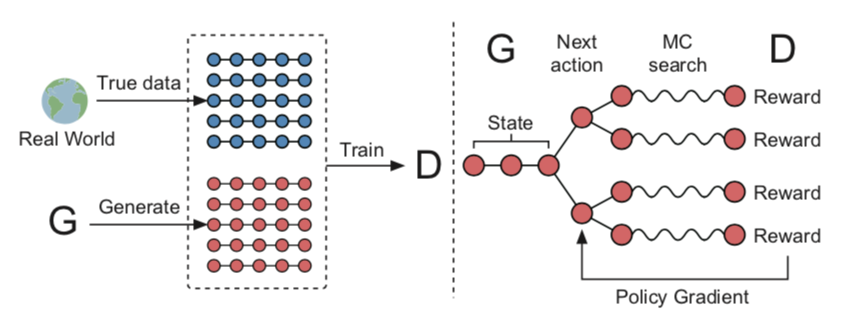
\includegraphics[scale=1]{1.png}\\
\noindent 生成器是LSTM神经网络,判别器是CNN网络,true data是由一个target LSTM网络生成的。
\subsubsection{预训练}
\noindent 预训练生成器是利用极大似然估计的方法,不需要考虑reward。\\
预训练判别器是先由生成器生成一批负样本,然后二分类,训练CNN网络。
\subsubsection{生成器的目标函数}
\noindent 生成器的目标是maximize expected end reward,即生成器生成了一句完整的句子后,我们希望尽可能使其所有tokens的reward之和最大。\\\\
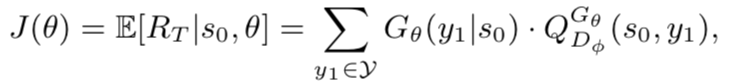
\includegraphics[scale=1]{2.png}\\
\noindent 其中RT可理解为一个完整句子的reward之和,s0表示初始状态,θ表示生成器的参数。后面的求和过程表示,每生成一个token,都要计算其生成该token的概率与其对应的reward值,那么两者相乘即表示生成该token的期望reward值,求和后即为该整句的期望reward值。生成器的目标就是不断maximize J。\\
reward是由后面判别器Dϕ决定的,下面需要解决的是如何求reward。\\\\
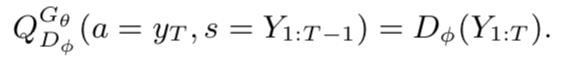
\includegraphics[scale=1]{3.png}\\\\\\\\
利用蒙特卡洛树搜索方法,因为只有是一个完整的句子,其判别器才能对其进行打分。例如在生成第t步的token时,后面的tokens是未知的,我们只能让生成器继续向后面生成token,直到生成一个完整的句子,然后在给判别器打分,为了让这个打分更有说服力,将这个过程重复N次取平均,由于生成器的随机性,每次生成的句子是不同的。\\\\
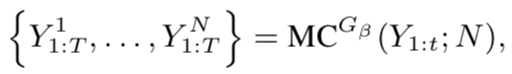
\includegraphics[scale=1]{4.png}\\
\noindent 式子左边表示sample出来的N个不同的完整句子。\\
综上所述,如下式。\\\\
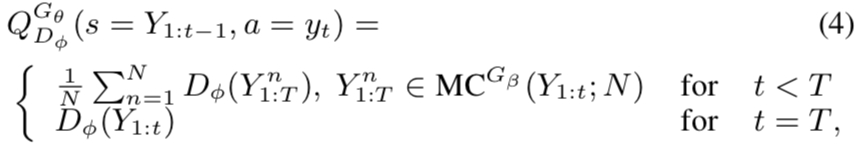
\includegraphics[scale=1]{5.png}\\
\noindent 打分过程大致如下:由于生成器是一个CNN网络,首先将input x(二分类的) reshape成一个四维的张量,然后通过各种卷积池化操作得到一个结果,然后再经过一个线性操作最终得到只有二维的张量,再做一个softmax操作得到ypred作为reward值。总地来说就是将该整句被判别器判别为真样本的概率作为该token的reward,判别为真样本的概率越大,当前步选择该token越正向。\\
这里reward的方式并不唯一,论文中的对比实验就用了blue指标作为reward来指导生成器的训练,这里也是可能可以创新的一个点。
\subsubsection{判别器的目标函数}
\noindent 判别器是一个CNN网络,喂给判别器的样本是一个二分类的样本,即有生成器生成的一批假样本,也有一批真样本,然后直接做个二分类,损失函数就是一个cross entropy。\\\\
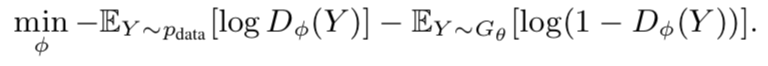
\includegraphics[scale=1]{6.png}
\subsubsection{策略梯度}
\noindent 利用梯度上升法更新生成器参数。\\
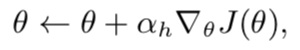
\includegraphics[scale=1]{0.png}\\
\noindent 对参数theta求导结果如下。\\
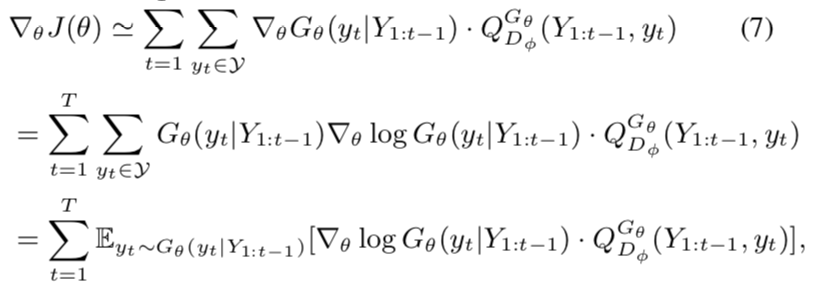
\includegraphics[scale=1]{7.png}
\subsubsection{算法概述}
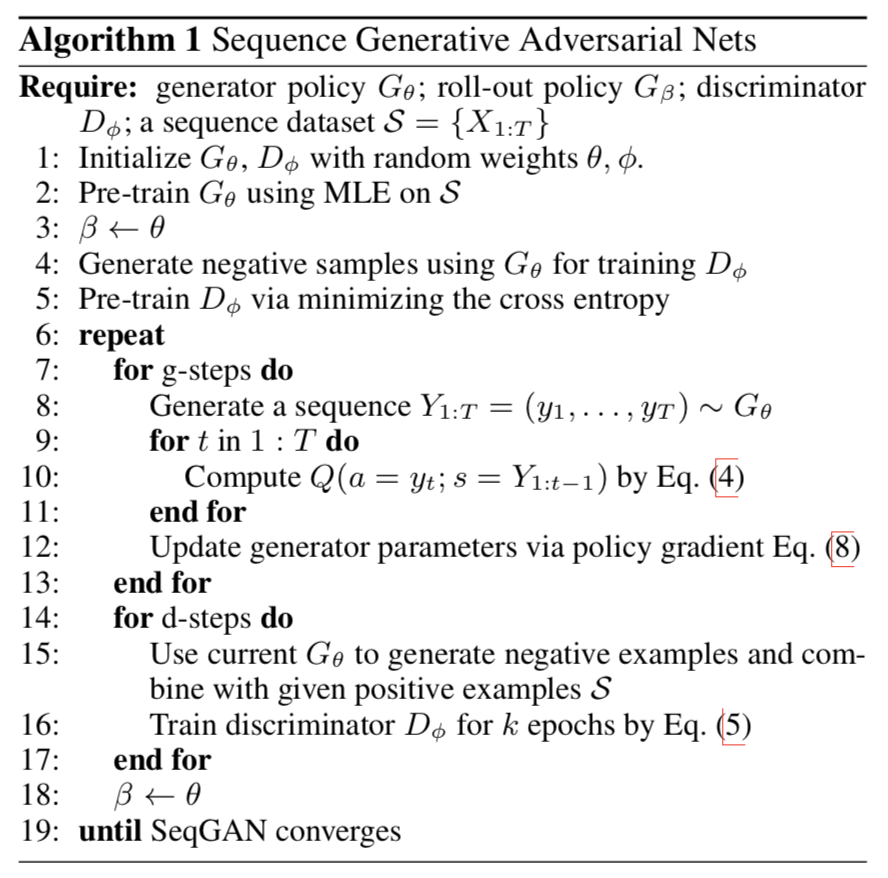
\includegraphics[scale=1]{8.png}\\\\\\
\noindent G-step中,利用生成器生成一批假样本,生成器每一步都是生成一个在词上的分布,我们以某种方式抽样一个token作为本步生成的token。在MLE作为目标函数时,我们需得到true data中当前步的token在当前生成分布中的概率,在SeqGAN中考虑的是当前步得到的 token在生成分布中的概率以及该token的reward,利用蒙特卡洛树搜索法得到每个token的reward。利用policy gradient更新生成器的参数。\\
D-step中,利用上面已经训完的生成器生成一批样本作为假样本,加上已有的一批真样本,作为训练数据,来训练一个二分类的判别器。
\subsection{个人想法}
\noindent GAN的生成器生成的序列需要喂给判别器,然后利用判别器来反向纠正生成器,这个时候梯度的微调不再适用在离散的数据上,并且梯度在回传时可能会有一些困难。SeqGAN中,生成器每生成一个token时,都会计算该token在生成分别中的概率,并且利用上一次训完的判别器计算出相应的reward,经过几轮的训练后,reward越大的token越正向,越容易生成,因此避免了判别器反向传递梯度给生成器。\\
GAN只能评估出整个生成序列的score和loss,不能够细化到去评估当前生成token的好坏和对后面生成的影响,SeqGAN模型将强化学习和对抗思想的结合,解决非连续序列生成的问题,产生可用于文本序列生成的模型。
\section{SeqGAN论文复现}
\noindent \\下一步计划是基于对论文算法的理解进行复现,届时应该会对论文和算法的理解上一层台阶,同时寻找GAN+RL的创新点。
	
\end{document}